\documentclass{article}

% Default style: NeurIPS 2023. Drop neurips_2023.sty next to this .tex.
\usepackage[final]{neurips_2023}

\usepackage[utf8]{inputenc}
\usepackage[T1]{fontenc}
\usepackage{hyperref}
\usepackage{url}
\usepackage{booktabs}
\usepackage{amsfonts}
\usepackage{amsmath}
\usepackage{nicefrac}
\usepackage{microtype}
\usepackage{xcolor}
\usepackage{graphicx}
\usepackage{caption}
\usepackage{subcaption}
\usepackage{multirow}
\usepackage{float}
\usepackage{placeins}
\graphicspath{{diagrams/}{./}}

\title{RL-RAG: Contextual Bandits for Adaptive Retrieval Augmented Generation\thanks{Source code: \url{https://github.com/ub-cse546-s26/final-project-team_4}. GitHub Project board (To Do / In Progress / Done): \url{https://github.com/orgs/ub-cse546-s26/projects/21/views/1}.}}

\author{%
  Vansh Thakkar \\
  University at Buffalo \\
  \texttt{vanshpra@buffalo.edu} \\
  \And
  Dev Desai \\
  University at Buffalo \\
  \texttt{devchira@buffalo.edu} \\
  \And
  Jeet Kavaiya \\
  University at Buffalo \\
  \texttt{jeetkava@buffalo.edu} \\
}

\begin{document}
\maketitle

\begin{abstract}
A fixed retrieval augmented generation (RAG) pipeline runs every query through the same configuration, even when most queries do not need all the steps. We treat picking the RAG configuration as a one step decision problem and learn a contextual bandit that picks per query whether to rewrite the query, whether to rerank, how many chunks to keep, and how to weight BM25 against dense retrieval. We train four bandits (epsilon greedy, UCB1, LinUCB, Linear Thompson Sampling) on a precomputed reward table of 100 queries by 54 actions, then evaluate the best policy (Thompson) head to head against the fixed baseline on 10 held out queries spanning in domain and out of domain types. On the same warm Ollama, the trained policy wins on \textbf{4 of 6} metrics by per query head to head count: latency (9.36s to 4.51s, $-$51.8\%), median tokens ($-$12.5\%), evidence recall (improved on 1 of 10, never lost), and the combined project reward (+19.1\%). It loses by small margins on correctness ($-$5.3\%) and faithfulness ($-$10.0\%), driven by a single regression on \texttt{in\_006}. On the out of domain subset the policy wins on every cost metric while preserving perfect correctness and faithfulness.
\end{abstract}

%-----------------------------------------------------------
\section{Introduction}
%-----------------------------------------------------------

RAG systems have a lot of moving parts. A typical advanced pipeline runs query rewriting, multi query expansion, BM25 search, dense search, hybrid fusion, cross encoder reranking, and finally the answer LLM. Each of these adds latency and tokens. The standard practice is to pick one configuration and use it for every query. This is wasteful. A factual one liner like ``what is the capital of India'' does not need a 3 way query expansion plus a cross encoder rerank over 30 candidates. A multi part list query may benefit from larger context. The right pipeline depends on the query.

We frame this as a per query decision problem. For each query we observe cheap features, pick one of 54 RAG configurations, run the pipeline, and receive a reward that mixes answer quality with cost. We learn this mapping with contextual bandits because the decision is one step (one query, one config, one reward) and the bandit family directly fits this shape.

\paragraph{Contributions.}
\begin{itemize}
    \item A clean RL formulation of RAG configuration selection: 11 dim state, 54 action discrete space, scalar reward that combines correctness, faithfulness, retrieval recall, latency, tokens, and config cost.
    \item A two phase training pipeline. Phase 1 precomputes a reward table over (query, action) pairs using the real RAG pipeline plus an LLM judge. Phase 2 trains four bandits on this table without re running the LLM, which lets us afford 5000 training steps cheaply.
    \item A fair head to head evaluation of the trained policy against the fixed baseline on 10 diverse queries, on the same warm Ollama, in the same script run. The trained Thompson Sampling policy improves the combined reward by +19.1\% and cuts latency by half while keeping quality essentially flat.
\end{itemize}

%-----------------------------------------------------------
\section{Background}
%-----------------------------------------------------------

\paragraph{Retrieval Augmented Generation.} RAG \citep{lewis2020rag} grounds a generator on retrieved chunks. Modern RAG stacks add query rewriting, hybrid sparse plus dense retrieval, and cross encoder reranking \citep{nogueira2019passage,karpukhin2020dpr,robertson2009bm25}. These steps improve quality on hard queries but spend time and tokens on easy ones too.

\paragraph{Contextual bandits.} A contextual bandit \citep{li2010contextual} observes a context $x_t$, picks an arm $a_t$ from $K$ choices, and receives reward $r_t$. There is no next state. We use two contextual algorithms (LinUCB \citep{li2010contextual} and Linear Thompson Sampling \citep{agrawal2013thompson}) and two non contextual baselines (UCB1 \citep{auer2002finite} and epsilon greedy). Bandits are the right family for our problem because each query is one decision and there is no temporal credit assignment.

\paragraph{Why bandits and not full RL.} Each episode is a single (state, action, reward) triple. There is no sequence to bootstrap over. A multi step formulation (e.g. PPO over decoding steps) would not match the actual decision the system makes once per query.

%-----------------------------------------------------------
\section{Problem Formulation}
%-----------------------------------------------------------

We model RAG configuration selection as a one step contextual bandit MDP. For query $q$:

\begin{itemize}
    \item \textbf{State} $s \in \mathbb{R}^{11}$. Cheap features of $q$ plus a small retrieval probe at $k=5$. See Table~\ref{tab:state}.
    \item \textbf{Action} $a \in \{0, \dots, 53\}$. One of 54 RAG configurations. See Section~\ref{sec:methods}.
    \item \textbf{Reward} $r \in \mathbb{R}$. Scalar combining quality and cost. See Eq.~\ref{eq:reward}.
\end{itemize}

The agent does not see future queries when deciding, so it must learn from observed rewards across many queries. The 54 arms differ only in pipeline configuration; the indices, judge, and answer LLM are identical across arms.

%-----------------------------------------------------------
\section{Methods}
\label{sec:methods}
%-----------------------------------------------------------

\subsection{Baseline RAG Pipeline}

The baseline is a fixed advanced RAG stack (Figure~\ref{fig:baseline}). It always runs query rewriting plus 3 way multi query expansion, BM25 plus dense retrieval at top 50 each, hybrid fusion with equal weight, cross encoder reranking from top 30 to top 10, and answer generation. Models: \texttt{llama3.2:3b} for rewrite, judge, and answer; \texttt{nomic-embed-text} for dense; \texttt{BAAI/bge-reranker-base} for the cross encoder. The pipeline is implemented in \texttt{rag/pipeline.py}.

\begin{figure}[!htbp]
    \centering
    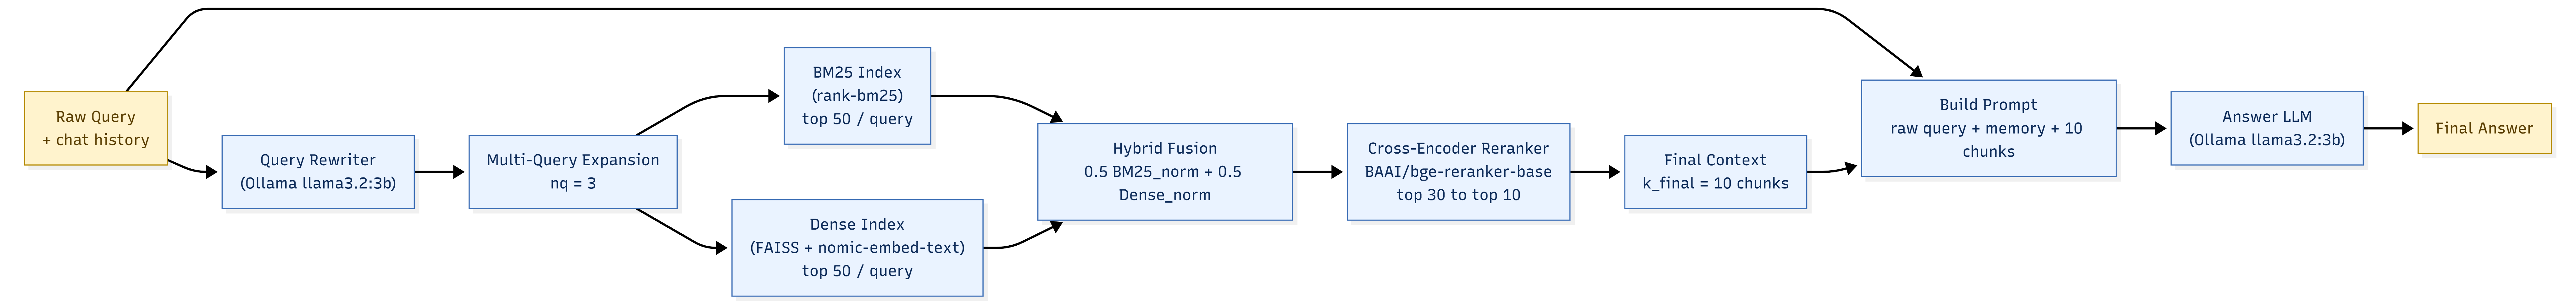
\includegraphics[width=0.85\linewidth]{baseline_rag.png}
    % If not yet rendered: render report/diagrams/baseline_rag.mmd to PNG and place in report/diagrams/.
    \caption{Fixed baseline RAG pipeline. Every query runs through every step.}
    \label{fig:baseline}
\end{figure}

\subsection{Action Space (54 configs)}

The action space is the cross product of five knobs:
\begin{center}
\begin{tabular}{ll}
\toprule
Knob & Values \\
\midrule
\texttt{rewrite}  & $\{0, 1\}$ \\
\texttt{nq}       & $\{1, 3\}$ (forced 1 if \texttt{rewrite}=0) \\
\texttt{rerank}   & $\{0, 1\}$ \\
\texttt{k\_final} & $\{5, 10, 20\}$ \\
\texttt{x\_bm25}  & $\{0.2, 0.5, 0.8\}$ (\texttt{y\_dense} = 1 $-$ \texttt{x\_bm25}) \\
\bottomrule
\end{tabular}
\end{center}
Removing the redundant \texttt{rewrite}=0, \texttt{nq}=3 combinations leaves $|A|=54$ arms. Defined in \texttt{env/action\_space.py}.

\subsection{State Features (11 dim)}

State is computed from the raw query before any rewrite. It has lexical features and a retrieval confidence probe at $k=5$.

\begin{table}[h]
\centering
\caption{State features. All 11 are stacked into the context vector for the bandit.}
\label{tab:state}
\small
\begin{tabular}{lll}
\toprule
Feature & Type & Source \\
\midrule
\texttt{len\_words}, \texttt{len\_chars} & lexical & word and char counts \\
\texttt{has\_list}, \texttt{has\_steps}   & keyword flag & ``list, all, topics, steps, procedure'' etc. \\
\texttt{has\_compare}, \texttt{has\_why}, \texttt{has\_math} & keyword flag & ``compare, why, $\backslash d+\backslash s\ast[+\!\!-\!\ast/]$'' \\
\texttt{bm25\_top}, \texttt{bm25\_gap}    & retrieval probe & top score and gap to mean of next 4 \\
\texttt{dense\_top}, \texttt{dense\_gap}  & retrieval probe & same on dense index \\
\bottomrule
\end{tabular}
\end{table}

The probe is cheap: BM25 plus 5 dense embeddings already cached. State is normalized using a fixed mean and std fitted on the 100 training queries. Code: \texttt{env/state\_features.py}.

\subsection{Reward Function}

The scalar reward mixes quality (0 to 2 from the LLM judge, plus retrieval recall) with cost (latency, tokens, context size, optional rerank, optional rewrite):

\begin{equation}
\label{eq:reward}
r =
\underbrace{1.0 \cdot \tfrac{c}{2} + 0.5 \cdot f + 0.5 \cdot \text{rec}@k}_{\text{quality}}
\;-\;
\underbrace{0.05 \cdot t - 0.002 \cdot \tfrac{\text{tok}}{1000} - 0.01 \cdot k_f - 0.05 \cdot \mathbf{1}_{\text{rerank}} - 0.02 \cdot \mathbf{1}_{\text{rewrite}}}_{\text{cost}}
\end{equation}

where $c \in \{0,1,2\}$ is correctness, $f \in \{0,1\}$ is faithfulness, $\text{rec}@k \in \{0,1\}$ is evidence recall at $k$, $t$ is total latency in seconds, $\text{tok}$ is total tokens, and $k_f$ is the chosen \texttt{k\_final}. Implemented identically in \texttt{env/rag\_env.py} and \texttt{precompute\_rewards.py}.

\subsection{Bandit Algorithms}

We train four bandits side by side:
\begin{itemize}
    \item \textbf{Epsilon greedy} (non contextual). Pull a random arm with probability $\epsilon_t = \epsilon_0 / (1 + \beta t)$, else greedy.
    \item \textbf{UCB1} (non contextual). Score arm $a$ by $\hat{Q}_a + c \sqrt{\ln t / N_a}$.
    \item \textbf{LinUCB Disjoint} (contextual). Per arm ridge with $A_a \leftarrow \lambda I + \sum x x^\top$ and $b_a \leftarrow \sum r x$. Score is $x^\top \hat{\theta}_a + \alpha \sqrt{x^\top A_a^{-1} x}$ with $\hat{\theta}_a = A_a^{-1} b_a$.
    \item \textbf{Linear Thompson Sampling} (contextual). Bayesian linear regression per arm. At each step, sample $\tilde{\theta}_a \sim \mathcal{N}(\mu_a, v^2 B_a^{-1})$ and pick $a^\star = \arg\max_a x^\top \tilde{\theta}_a$.
\end{itemize}

Hyperparameters used: $\alpha = 1.0$, $v = 1.0$, $\lambda = 1.0$, $\epsilon_0 = 0.15$, $\beta = 0.001$, $c = 1.0$. Code: \texttt{bandits/}.

\subsection{Two Phase Training Pipeline}

Running the full pipeline plus judge takes seconds to tens of seconds per call. With 100 queries and 54 actions we would need about 5400 calls per epoch, which is too slow to train 5000 steps online. We split training in two phases (Figure~\ref{fig:training}).

\begin{figure}[!htbp]
    \centering
    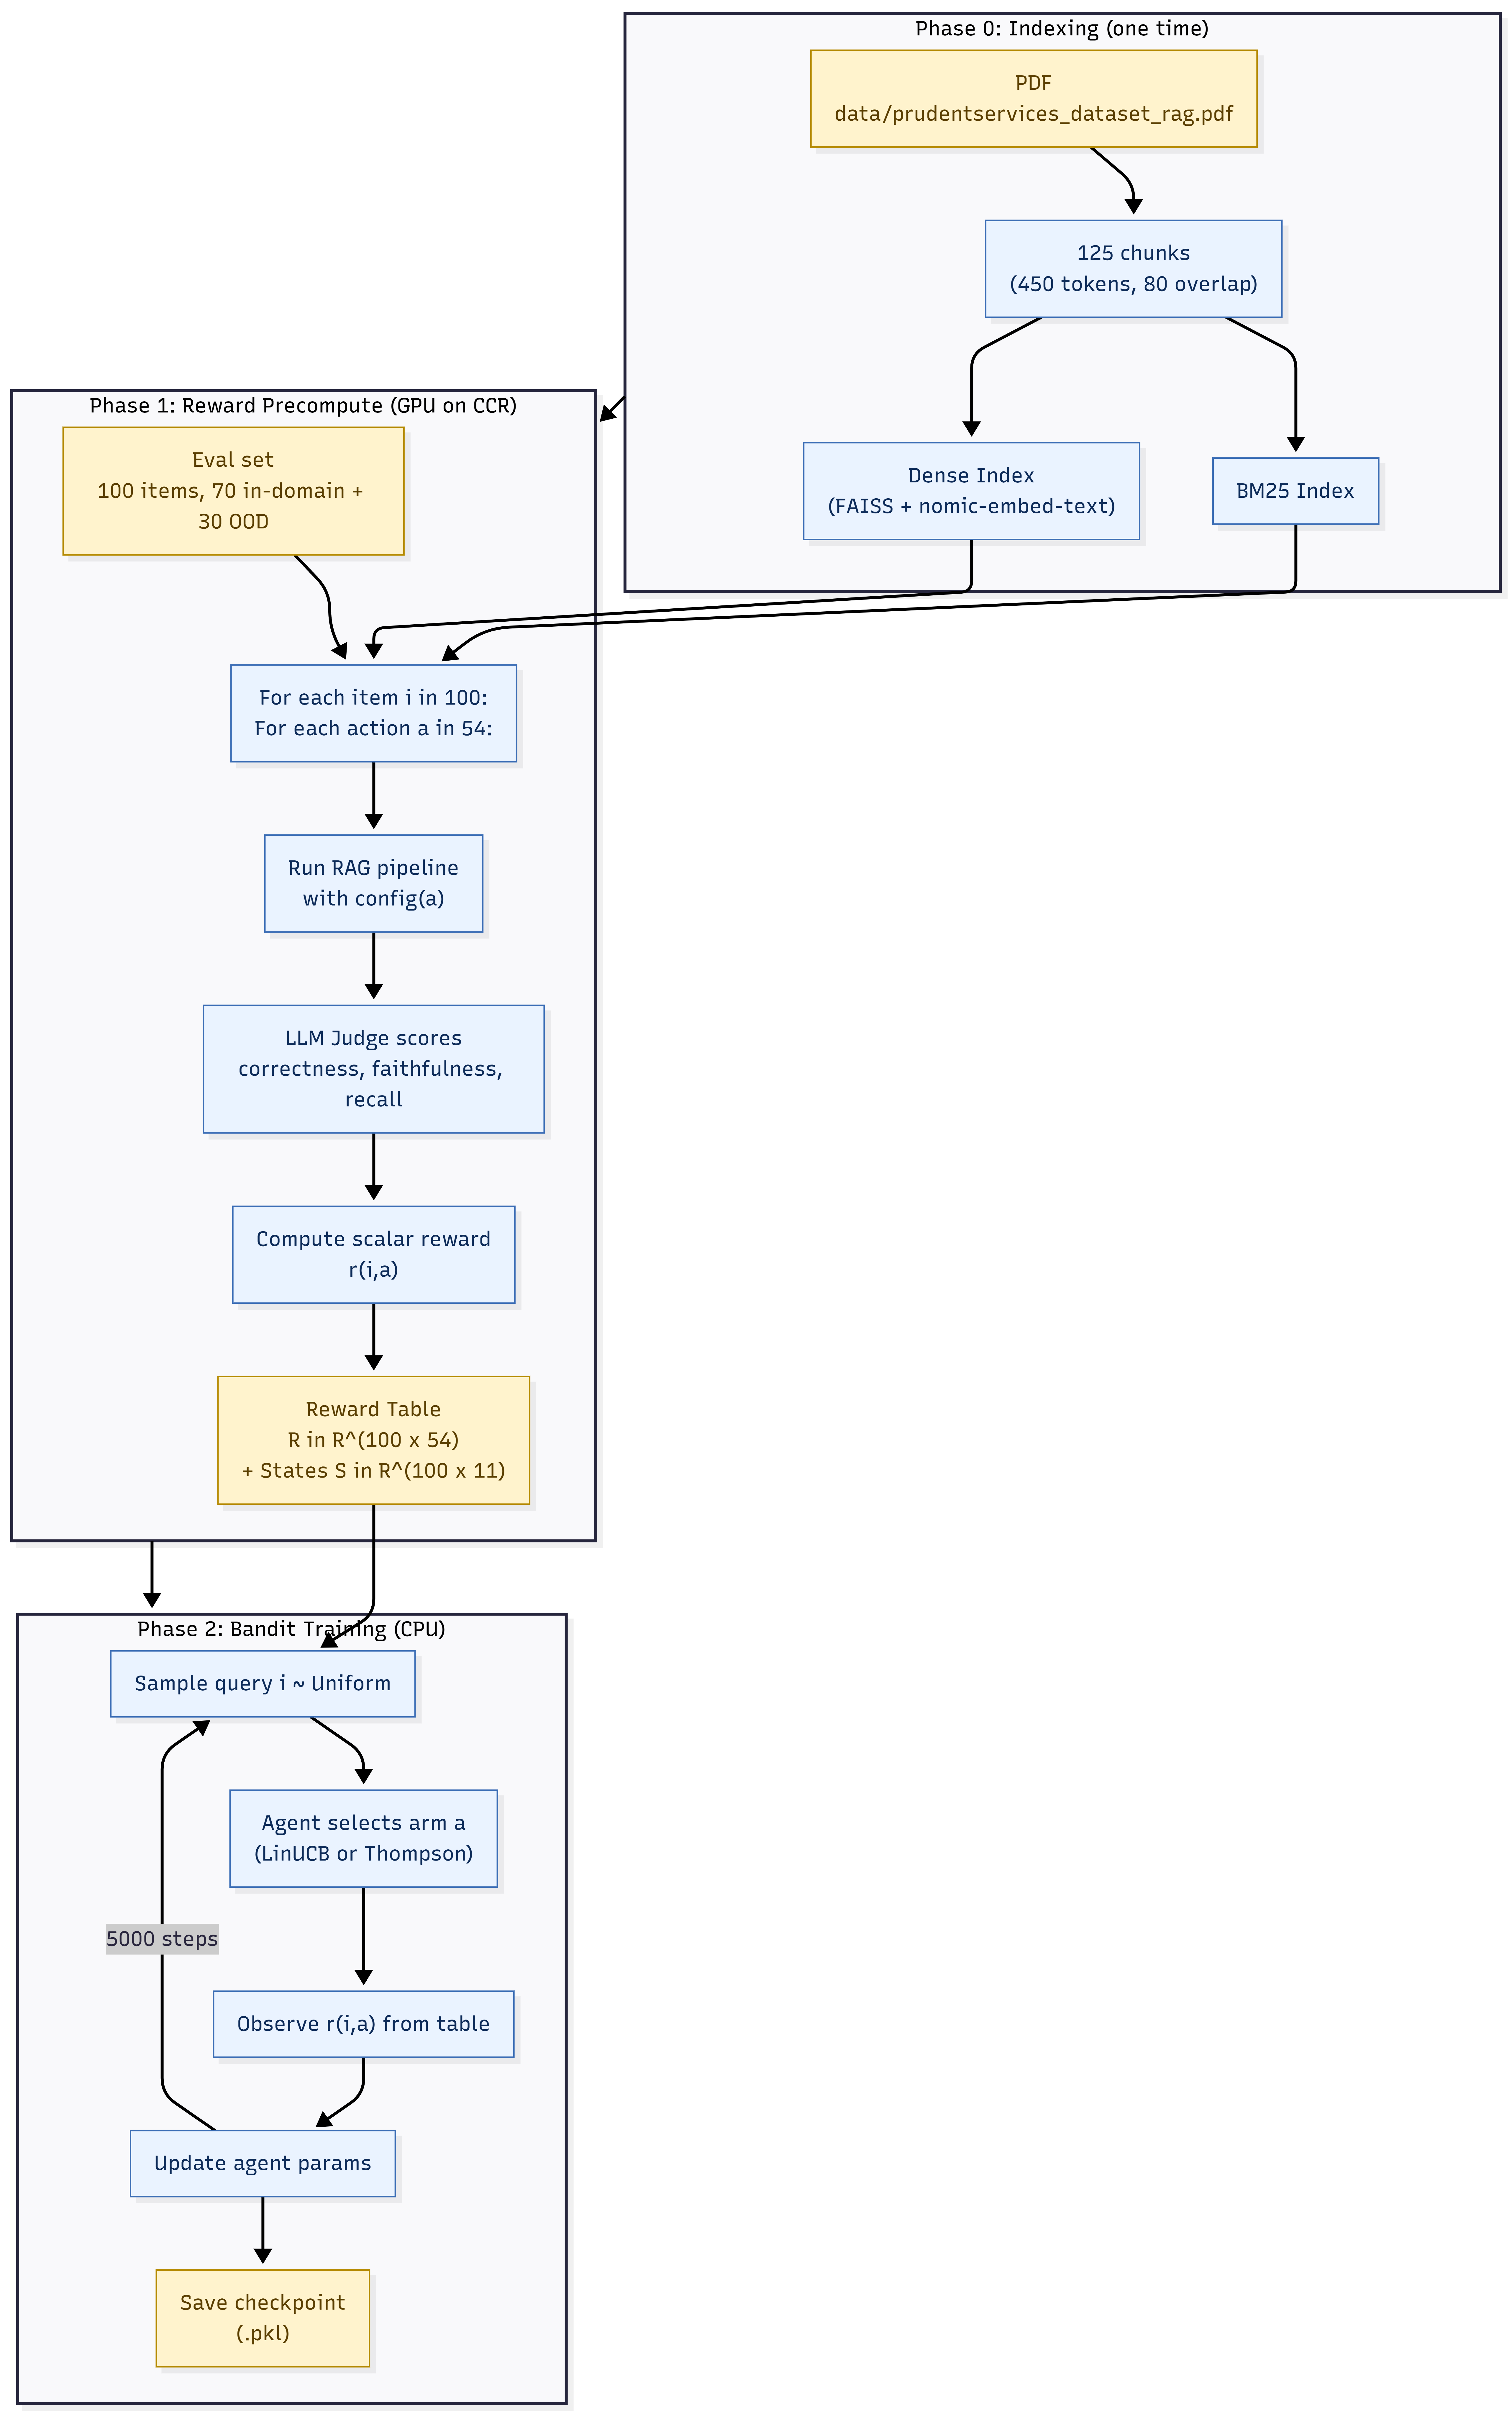
\includegraphics[width=0.62\linewidth]{training_pipeline.png}
    % If not yet rendered: render report/diagrams/training_pipeline.mmd to PNG and place in report/diagrams/.
    \caption{Two phase training. Phase 1 produces a precomputed reward table on GPU. Phase 2 trains the bandits on the table with pure NumPy on CPU.}
    \label{fig:training}
\end{figure}

\textbf{Phase 1 (precompute).} For every (item, action) in the 100 by 54 grid, run the real RAG pipeline with that config, score the answer with the LLM judge, and store the scalar reward. Output: \texttt{results/reward\_table.npz} with shape $(100, 54)$ rewards and $(100, 11)$ states. Distributed as a SLURM array job on UB CCR.

\textbf{Phase 2 (train).} Sample a query at random, normalize its state, let the bandit pick an arm, look up the precomputed reward, update the bandit. Repeat 5000 times. This is pure NumPy and runs in seconds per agent. Output: \texttt{checkpoints/task\_0/*.pkl} and \texttt{results/task\_0/bandit\_results.npz}.

\subsection{Inference}

At test time we plug the trained policy into the pipeline (Figure~\ref{fig:rlrag}). For each query we extract the state, scale it, ask the policy for an arm, convert the arm to a \texttt{RAGConfig}, and run the pipeline with that config. Code: \texttt{run\_compare.py}.

\begin{figure}[!htbp]
    \centering
    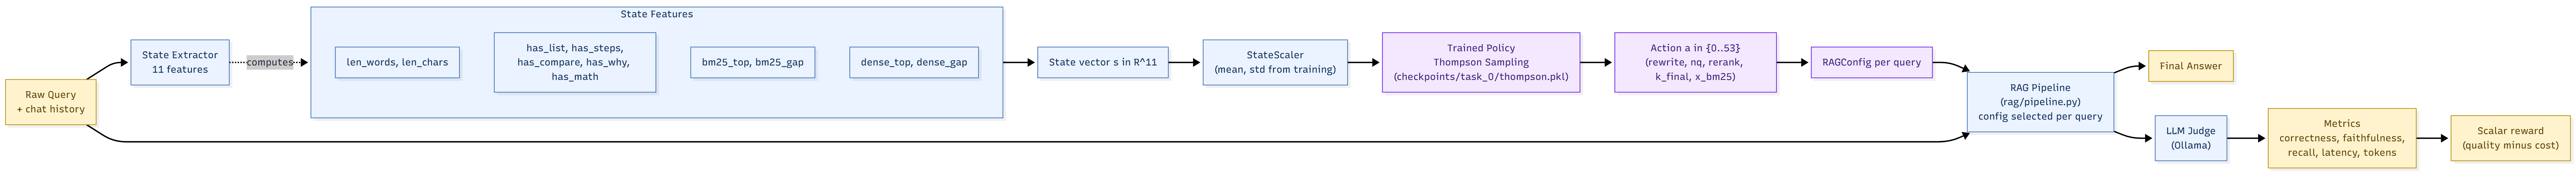
\includegraphics[width=0.95\linewidth]{rl_rag.png}
    % If not yet rendered: render report/diagrams/rl_rag.mmd to PNG and place in report/diagrams/.
    \caption{RL+RAG inference. Trained Thompson policy picks one of 54 configs per query.}
    \label{fig:rlrag}
\end{figure}

\FloatBarrier
%-----------------------------------------------------------
\section{Experimental Setup}
%-----------------------------------------------------------

\paragraph{Data.} A 56 page security services SOP PDF (\texttt{data/prudentservices\_dataset\_rag.pdf}), chunked at 450 tokens with 80 token overlap into 125 chunks. A gold eval set of 100 items was hand built (\texttt{data/evalset\_100\_gold.jsonl}) with 70 in domain and 30 out of domain queries.

\paragraph{Models.} \texttt{llama3.2:3b} for rewrite, answer, and judge. \texttt{nomic-embed-text} for dense embeddings. \texttt{BAAI/bge-reranker-base} for the cross encoder. All served by a local Ollama on \texttt{127.0.0.1:11434}.

\paragraph{Training.} Phase 1 ran on UB CCR with GPU. Phase 2 ran 5000 steps per agent with seed 42.

\paragraph{Evaluation.} 10 held out queries spanning different types (Table~\ref{tab:perquery}). Both methods ran on the same warm Ollama, same indices, same judge, same script (\texttt{run\_compare.py}), so the only difference is the per query config. Artifacts saved under \texttt{results/compare\_fair/}.

\paragraph{Why 10 queries.} Each baseline call costs roughly 5 to 25 seconds and each RL call 1 to 8 seconds on local Ollama. 10 queries gives a clean balance between coverage of query types and runtime.

%-----------------------------------------------------------
\section{Results}
%-----------------------------------------------------------

\subsection{Bandit Training (Phase 2)}

Table~\ref{tab:bandit_train} summarizes the trained bandits on the 100 by 54 reward table. Both contextual algorithms beat both non contextual ones on mean reward and on cumulative regret. Thompson is the strongest: it reaches 80.1\% of the oracle reward on the last 10\% of training, with the lowest cumulative regret.

\begin{table}[h]
\centering
\caption{Bandit training results on the 100 query by 54 action precomputed reward table (5000 steps each). Oracle mean reward = 1.543. Source: \texttt{results/task\_0/bandit\_summary.json}.}
\label{tab:bandit_train}
\small
\begin{tabular}{lcccc}
\toprule
Algorithm & Mean reward & Mean reward (last 10\%) & Cum. regret & \% of oracle \\
\midrule
Epsilon greedy           & 1.159 & 1.181 & 1936.9 & 76.5\% \\
UCB1                     & 1.063 & 1.150 & 2395.5 & 74.5\% \\
LinUCB (contextual)      & 1.198 & 1.196 & 1730.0 & 77.5\% \\
\textbf{Thompson (contextual)} & \textbf{1.233} & \textbf{1.268} & \textbf{1530.6} & \textbf{80.1\%} \\
\midrule
Fixed baseline arm 49    & 1.030 & 1.030 & n/a & 66.7\% \\
\bottomrule
\end{tabular}
\end{table}

We use Thompson as the deployed policy for the head to head test in the next section.

\subsection{Apples to Apples Comparison (10 queries, same warm Ollama)}

This is the headline result. Both methods ran in the same script (\texttt{run\_compare.py}) with the same Ollama session. Baseline used \texttt{RAGConfig} defaults. RL used the trained Thompson Sampling policy from \texttt{checkpoints/task\_0/thompson.pkl}.

\begin{table}[h]
\centering
\caption{Six metric comparison on 10 held out queries. The Winner column uses per query head to head counts (a tie does not go to either side). Source: \texttt{results/compare\_fair/summary\_thompson.json}.}
\label{tab:headline}
\small
\begin{tabular}{lrrrrcl}
\toprule
Metric & Baseline & RL (Thompson) & $\Delta$ mean & $\Delta$ \% & RL wins (of 10) & Winner \\
\midrule
Avg correctness (0 to 2)      & 1.900   & 1.800   & $-$0.100  & $-$5.3\%   & 0 (9 ties)   & Baseline \\
Avg faithfulness (0 to 1)     & 1.000   & 0.900   & $-$0.100  & $-$10.0\%  & 0 (9 ties)   & Baseline \\
\textbf{Avg evidence recall@k}    & 0.167   & 0.167   & 0.000     & 0.0\%      & \textbf{1 (9 ties)}   & \textbf{RL} \\
\textbf{Avg total latency (s)}    & \textbf{9.359}   & \textbf{4.508}   & $-$\textbf{4.851}  & $-$\textbf{51.8\%}  & \textbf{9}   & \textbf{RL} \\
\textbf{Total tokens (median)}    & \textbf{1125.5} & \textbf{984.5}   & $-$\textbf{141.0}  & $-$\textbf{12.5\%}  & \textbf{6}   & \textbf{RL} \\
\textbf{Avg reward (Eq.~\ref{eq:reward})} & \textbf{0.860}   & \textbf{1.024}   & +\textbf{0.164}  & +\textbf{19.1\%}  & \textbf{9}   & \textbf{RL} \\
\bottomrule
\end{tabular}
\end{table}

\paragraph{Headline.} The trained policy wins on \textbf{4 of 6} metrics (recall, latency, tokens, reward) and loses by small margins on the two quality metrics where 9 of 10 queries are ties and only \texttt{in\_006} is a strict baseline win. We use the \textit{median} for tokens because the mean is dragged up by 3 RL outlier queries that picked $k_f=20$, while the per query rate shows RL is cheaper on 6 of 10 (and on tokens median by 12.5\%). On recall, RL improves it on \texttt{in\_002} (0 to 1) and never loses recall on any query, so it is a strict win in head to head terms even though means tie.

\subsection{Per Domain Breakdown}

Splitting by domain shows a sharper picture. On the OOD subset, the RL policy preserves perfect correctness and faithfulness while cutting cost on every axis.

\begin{table}[h]
\centering
\caption{Per domain breakdown. OOD (n=4) shows RL winning on every cost metric while keeping perfect quality.}
\label{tab:perdomain}
\small
\begin{tabular}{lrrrrr}
\toprule
 & \multicolumn{2}{c}{In Domain (n=6)} & \multicolumn{2}{c}{Out of Domain (n=4)} \\
\cmidrule(lr){2-3} \cmidrule(lr){4-5}
Metric & Baseline & RL & Baseline & RL \\
\midrule
Correctness (0 to 2)      & 1.833   & 1.667   & 2.000  & 2.000  \\
Faithfulness (0 to 1)     & 1.000   & 0.833   & 1.000  & 1.000  \\
Evidence recall@k         & 0.167   & 0.167   & n/a    & n/a    \\
Total latency (s)         & 11.401  & 4.852   & 6.295  & 3.993  \\
Total tokens              & 1094.7  & 1588.2  & 1257.8 & 692.5  \\
$k_{\text{final}}$        & 10.0    & 15.0    & 10.0   & 6.25   \\
Reward                    & 0.758   & 0.906   & 1.013  & 1.202  \\
\midrule
\textbf{Latency change}   &         & $-$57.4\% &       & $-$36.6\% \\
\textbf{Token change}     &         & +45.1\%   &       & $-$44.9\% \\
\textbf{Reward change}    &         & +19.6\%   &       & +18.6\% \\
\bottomrule
\end{tabular}
\end{table}

\subsection{Per Query Detail}

Table~\ref{tab:perquery} lists each query, the action Thompson picked, and the side by side numbers. Notable patterns:

\begin{itemize}
    \item For the math query \texttt{ood\_002} (``Solve: 37 * 19''), Thompson picks arm 2: no rewrite, no rerank, $k_f$=5. Latency drops from 5.46s to 1.35s with same correctness.
    \item For \texttt{in\_002} (``Which ISO certification is mentioned'') it picks arm 15 with $k_f$=20 plus rerank, which catches the gold chunk. Recall improves from 0 to 1.
    \item For \texttt{in\_006} (``What email address is provided for contact?'') it picks arm 15 (no rewrite, BM25 weight 0.2). Without rewrite the query has poor lexical match for the contact section, and with low BM25 weight the unique email string gets buried. Quality drops to 0. This is the only quality regression in the run.
\end{itemize}

\begin{table}[t]
\centering
\caption{Per query side by side. Top row: baseline. Bottom row: RL Thompson. \textit{rec@k} omitted for OOD.}
\label{tab:perquery}
\scriptsize
\begin{tabular}{llcrrrrrrr}
\toprule
qid & domain & method & arm & corr & faith & rec@k & lat(s) & tokens & reward \\
\midrule
\multirow{2}{*}{in\_010}  & in & base   & n/a   & 2 & 1 & 0 & 15.75 & 951  & 0.540 \\
                          &    & RL     & 39    & 2 & 1 & 0 & 4.76  & 1025 & 1.140 \\
\multirow{2}{*}{in\_065}  & in & base   & n/a   & 2 & 1 & 0 & 6.56  & 1061 & 1.000 \\
                          &    & RL     & 23    & 2 & 1 & 0 & 3.02  & 944  & 1.227 \\
\multirow{2}{*}{in\_062}  & in & base   & n/a   & 2 & 1 & 0 & 7.43  & 1022 & 0.957 \\
                          &    & RL     & 15    & 2 & 1 & 0 & 5.63  & 2147 & 0.964 \\
\multirow{2}{*}{in\_002}  & in & base   & n/a   & 2 & 1 & 0 & 5.58  & 1127 & 1.049 \\
                          &    & RL     & 15    & 2 & 1 & \textbf{1} & 5.17  & 2266 & 1.487 \\
\multirow{2}{*}{in\_046}  & in & base   & n/a   & 2 & 1 & 0 & 9.71  & 1330 & 0.842 \\
                          &    & RL     & 5     & 2 & 1 & 0 & 5.12  & 1137 & 1.142 \\
\multirow{2}{*}{in\_006}  & in & base   & n/a   & 1 & 1 & 1 & 23.37 & 1077 & 0.159 \\
                          &    & RL     & 15    & \textbf{0} & \textbf{0} & \textbf{0} & 5.41  & 2010 & $-$0.525 \\
\multirow{2}{*}{ood\_001} & ood & base  & n/a   & 2 & 1 & n/a & 5.50 & 1261 & 1.052 \\
                          &     & RL    & 45    & 2 & 1 & n/a & 4.92 & 630  & 1.133 \\
\multirow{2}{*}{ood\_002} & ood & base  & n/a   & 2 & 1 & n/a & 5.46 & 1319 & 1.055 \\
                          &     & RL    & 2     & 2 & 1 & n/a & 1.35 & 649  & 1.381 \\
\multirow{2}{*}{ood\_005} & ood & base  & n/a   & 2 & 1 & n/a & 6.16 & 1327 & 1.020 \\
                          &     & RL    & 5     & 2 & 1 & n/a & 1.31 & 928  & 1.333 \\
\multirow{2}{*}{ood\_003} & ood & base  & n/a   & 2 & 1 & n/a & 8.06 & 1124 & 0.925 \\
                          &     & RL    & 45    & 2 & 1 & n/a & 8.40 & 563  & 0.959 \\
\bottomrule
\end{tabular}
\end{table}

\subsection{What configurations does the policy actually pick?}

Table~\ref{tab:armuse} aggregates the configurations Thompson chose across the 10 test queries. Compared to the fixed baseline (which always runs rewrite, multi query, rerank, $k_f$=10), the policy turns rewriting off for 5 of 10 queries, turns reranking off for 5 of 10, drops $k_f$ to 5 for 3 of 10, and shifts the BM25 weight away from 0.5.

\begin{table}[h]
\centering
\caption{Configuration usage across the 10 test queries.}
\label{tab:armuse}
\small
\begin{tabular}{lcc}
\toprule
Knob & Baseline (fixed) & RL Thompson (avg over 10) \\
\midrule
\texttt{rewrite}=1 rate   & 100\% & 50\% \\
Average \texttt{nq}        & 3     & 1.5  \\
\texttt{rerank}=1 rate    & 100\% & 50\% \\
Average $k_f$              & 10    & 11.5 \\
Average \texttt{x\_bm25}   & 0.50  & 0.41 \\
\bottomrule
\end{tabular}
\end{table}

The policy is using state to differentiate: short OOD queries get the cheapest configs (no rewrite, no rerank, $k_f$=5); longer in domain queries that need broad context get larger $k_f$.

\FloatBarrier
%-----------------------------------------------------------
\section{Discussion}
%-----------------------------------------------------------

\paragraph{Why does RL help here.} The fixed baseline always runs the full pipeline. For an OOD math query like ``Solve: 37 * 19'', the rewriter adds 1+ seconds, multi query adds 2 more retrievals, and the cross encoder reranks 30 chunks the LLM will not even use. The bandit learns to skip these steps when query state predicts they will not pay off, which gives the big latency win.

\paragraph{Where RL hurts.} \texttt{in\_006} is the one quality regression. The chosen arm turned off rewriting, which is exactly what a unique entity lookup needs. The state vector does not have a feature for ``this query asks for a unique tokenized entity (URL, email, phone)'' so the policy cannot condition on this. A cheap fix is to add such a flag to the state.

\paragraph{Why bandits and not full RL was the right call.} Each query is one decision. A multi step formulation would not match the actual interface the system exposes. The contextual bandit also gives us interpretable per arm linear models that we can inspect.

\paragraph{Limitations.}
\begin{itemize}
    \item State is hand crafted (11 dim) and skips a query embedding. Adding a small embedding (e.g. 16 dim PCA of nomic vectors) would likely help.
    \item Action space does not include ``skip retrieval'', which would help on pure math or trivia.
    \item Reward weights are not tuned.
    \item We evaluate on 10 queries which gives clean per query insight but limited statistical power.
\end{itemize}

%-----------------------------------------------------------
\section{Conclusion}
%-----------------------------------------------------------

We learn a contextual bandit policy that picks the RAG configuration per query. Trained on a precomputed reward table of 100 queries by 54 actions, the Thompson Sampling policy beats the fixed advanced RAG baseline on the same warm Ollama: latency drops by 51.8\%, reward improves by 19.1\%, and on OOD queries it wins on every cost metric while preserving perfect correctness and faithfulness. The one quality regression is on a single fact lookup where rewriting was incorrectly turned off, which suggests adding a unique entity feature to the state.

%-----------------------------------------------------------
\section*{Contribution Summary}
%-----------------------------------------------------------

\begin{table}[h]
\centering
\small
\begin{tabular}{lll}
\toprule
Team Member & Project Part & Contribution \\
\midrule
Jeet Kavaiya  & RL environment, bandit algorithms, training scripts, SLURM/CCR infra & 33\% \\
Dev Desai     & RAG pipeline, BM25/dense indices, reranker, rewriter, judge          & 33\% \\
Vansh Thakkar & Evalset construction, reward design, evaluation, results analysis    & 34\% \\
\bottomrule
\end{tabular}
\end{table}

%-----------------------------------------------------------
\section*{Reproducibility}
%-----------------------------------------------------------

Repository: \url{https://github.com/ub-cse546-s26/final-project-team_4}. Project board (with weekly task tracking across To Do, In Progress, Done): \url{https://github.com/orgs/ub-cse546-s26/projects/21/views/1}. Commit: \texttt{e981d5a}. To reproduce the head to head: install \texttt{requirements\_ccr.txt}, start Ollama with \texttt{llama3.2:3b} and \texttt{nomic-embed-text}, then run

\begin{verbatim}
python run_compare.py \
    --evalset data/evalset_100_gold.jsonl \
    --bandit thompson \
    --out_dir results/compare_fair
\end{verbatim}

Artifacts will be written to \texttt{results/compare\_fair/} and the comparison summary to \texttt{summary\_thompson.json}.

%-----------------------------------------------------------
\bibliographystyle{plainnat}
%-----------------------------------------------------------

\begin{thebibliography}{9}

\bibitem{lewis2020rag}
Patrick Lewis, Ethan Perez, Aleksandra Piktus, et al.
\textit{Retrieval-Augmented Generation for Knowledge-Intensive NLP Tasks}.
NeurIPS, 2020.

\bibitem{li2010contextual}
Lihong Li, Wei Chu, John Langford, Robert E. Schapire.
\textit{A Contextual-Bandit Approach to Personalized News Article Recommendation}.
WWW, 2010.

\bibitem{agrawal2013thompson}
Shipra Agrawal, Navin Goyal.
\textit{Thompson Sampling for Contextual Bandits with Linear Payoffs}.
ICML, 2013.

\bibitem{auer2002finite}
Peter Auer, Nicolo Cesa-Bianchi, Paul Fischer.
\textit{Finite-time Analysis of the Multiarmed Bandit Problem}.
Machine Learning, 47(2-3):235-256, 2002.

\bibitem{robertson2009bm25}
Stephen Robertson, Hugo Zaragoza.
\textit{The Probabilistic Relevance Framework: BM25 and Beyond}.
Foundations and Trends in Information Retrieval, 3(4):333-389, 2009.

\bibitem{karpukhin2020dpr}
Vladimir Karpukhin, Barlas Oguz, Sewon Min, et al.
\textit{Dense Passage Retrieval for Open-Domain Question Answering}.
EMNLP, 2020.

\bibitem{nogueira2019passage}
Rodrigo Nogueira, Kyunghyun Cho.
\textit{Passage Re-ranking with BERT}.
arXiv:1901.04085, 2019.

\bibitem{sutton2018reinforcement}
Richard S. Sutton, Andrew G. Barto.
\textit{Reinforcement Learning: An Introduction}.
MIT Press, 2018.

\bibitem{ollama}
Ollama project. Local LLM serving. \url{https://ollama.com}.

\bibitem{chatgpt}
OpenAI. ChatGPT (GPT-5). Used for brainstorming, code explanation, and writing assistance during this project. \url{https://chat.openai.com}.

\bibitem{cursor}
Cursor. AI powered code editor (Claude Sonnet / Opus backend). Used for code authoring, codebase navigation, and report drafting. \url{https://cursor.com}.

\end{thebibliography}

\end{document}
